\section{Opgaver fra testen}

\subsection{Opgave 1}
\begin{align*}
3+2 = 5
\end{align*}

\subsection{Opgave 2}
\begin{align*}
7-4 = 3
\end{align*}

\subsection{Opgave 3}
\begin{align*}
3-11 = -8
\end{align*}

\subsection{Opgave 4}
Tegn et koordinatsystem og indsæt punkterne (0,0) (1,2) (3,4) (-3,-2)

Et punkts første koordinat beskriver hvor vi befinder os på x-aksen mens et punkts andet koordinat beskriver hvor vi befinder os på y-aksen. Det første punkt (0,0) fortæller os at vi befinder os på x-aksen ved $x = 0$ og på y-aksen ved $y = 0$. Punkterne kan ses indtegnet på nedenstående koordinatsystem

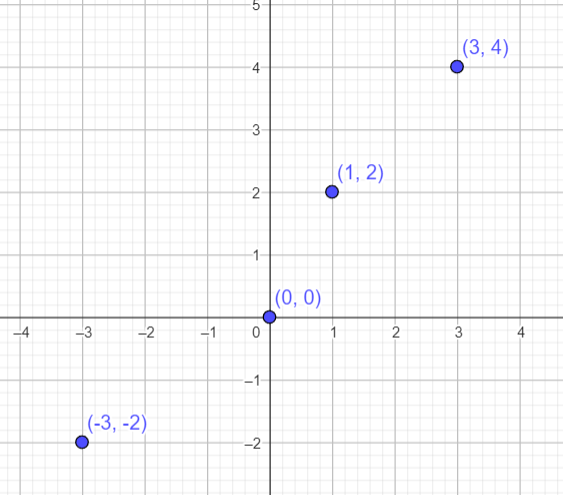
\includegraphics[scale=0.6]{img_19}



\subsection{Opgave 5}
Tegn et koordinatsystem og indtegn følgende rette linjer

$y = 3x+2$

$y = -\frac{1}{2}x-1$

For at indtegne en ret linje i et koordinatsystem aflæser vi først linjens hældning og linjens skæring med y-aksen. 
Den første linje $y = 3x+2$ har en hældning på 3 og skærer y-aksen i 2. Når vi har disse oplysninger, sætter vi først et punkt der hvor linjen skærer y-aksen. Dette kan ses på billedet nedenfor

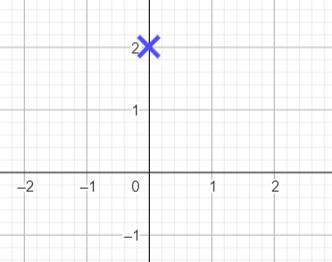
\includegraphics[scale=0.6]{img_20}


Derefter bruger vi den aflæste hældning 3 til at sætte det næste punkt. Vi går 1 hen ad x-aksen og 3 op ad y-aksen da linjens hældning er 3 og sætter det næste punkt. Dette er illustreret på nedenstående billede

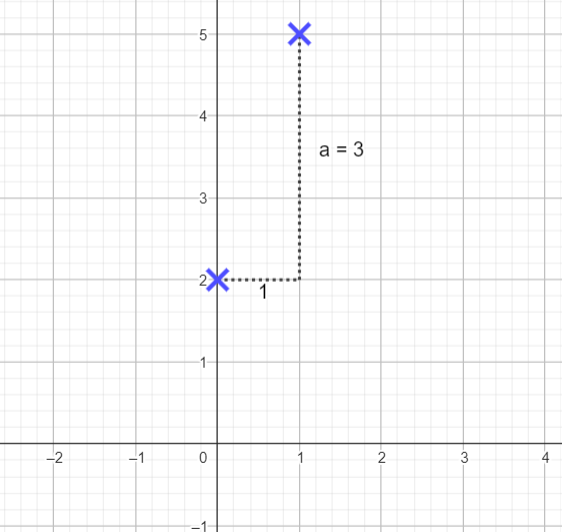
\includegraphics[scale=0.6]{img_21}

Ovenstående procedure gentages 1 gang mere hvorefter vi nu har 3 punkter i vores koordinatsystem. Forbinder vi disse 3 punkter med en ret linje har vi nu indtegnet vores rette linje i koordinatsystemet som kan ses nedenfor

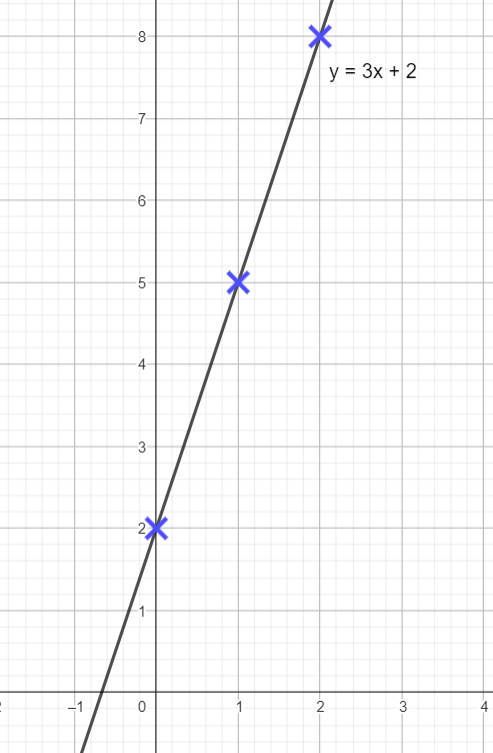
\includegraphics[scale=0.6]{img_22}

Som vi kan se på billedet stemme linjens ligning overens med den rette linje $y=3x+2$ som vi har indtegnet i koordinatsystemet.


For at indtegne den anden rette linje $-\frac{1}{2}x-1$ aflæser vi først linjens hældning og skæring med y-aksen. Linjens hældning er $-\frac{1}{2}$ og skærer y-aksen i -1. Vi indtegner det første punkt der hvor linjen skærer y-aksen. Dette kan ses på nedenstående billede.

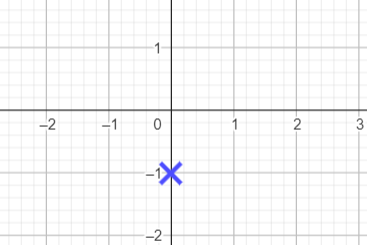
\includegraphics[scale=0.6]{img_23}

Derefter bruger vi den aflæste hældning $-\frac{1}{2}$ til at sætte det næste punkt. Vi går 1 hen ad x-aksen og $\frac{1}{2}$ ned ad y-aksen da linjens hældning er $-\frac{1}{2}$ og sætter det næste punkt. Dette er illustreret på nedenstående billede

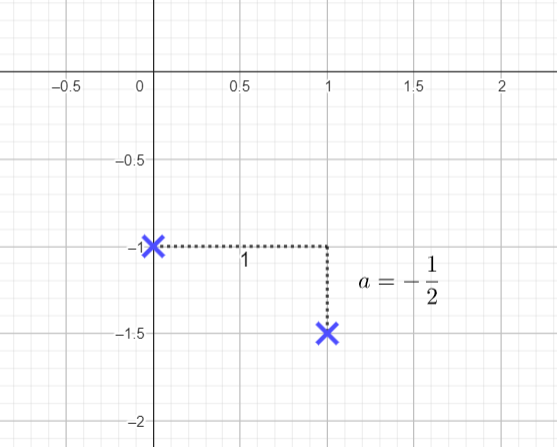
\includegraphics[scale=0.6]{img_24}

Ovenstående procedure gentages 1 gang mere hvorefter vi nu har 3 punkter i vores koordinatsystem. Forbinder vi disse 3 punkter med en ret linje har vi nu indtegnet vores rette linje i koordinatsystemet som kan ses nedenfor

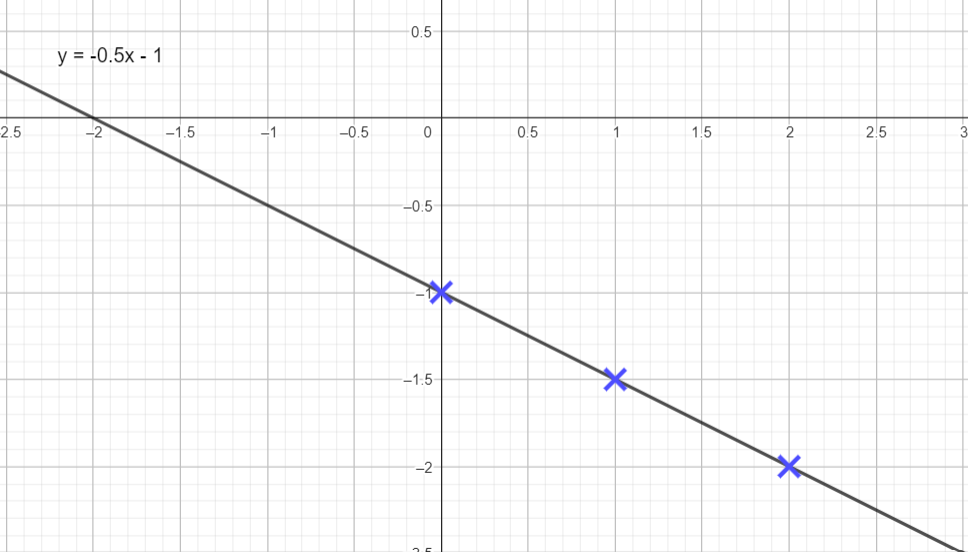
\includegraphics[scale=0.5]{img_25}

Som vi kan se på billedet stemme linjens ligning overens med den rette linje $y=- \frac{1}{2}x-1$ som vi har indtegnet i koordinatsystemet.





\subsection{Opgave 6}

Vi har en ret linje $y = 3x+4$

Udfyld sildebenet

\begin{tabular}{|c|c|c|c|c|}
\hline
X & -1 & 0 & 1 & 2 \\\hline
Y &  &  &  & \\\hline
\end{tabular}

og tegn punkterne ind i et koordinatsystem.


For at udfylde sildebenet skal vi altså beregne de tilsvarende y-værdier til de givne x-værdier. Dette gør vi ved at indsætte x-værdierne på x's plads i den rette linje $y = 3x +4$. For x-værdierne får vi de følgende y-værdier.

\begin{align*}
Y &= 3\cdot (-1) + 4 =-3 + 4 = 1 \\
Y &= 3\cdot 0 + 4 = 0 + 4 = 4\\
Y &= 3\cdot 1 + 4 = 3 + 4 = 7\\
Y &= 3\cdot 2 + 4 = 6 + 4 = 10
\end{align*}

Det færdige sildeben bliver derfor 

\begin{tabular}{|c|c|c|c|c|}
\hline
X & -1 & 0 & 1 & 2 \\\hline
Y & 1 & 4 & 7 & 10\\\hline
\end{tabular}

For at indtegne punkterne i et koordinatsystem er hver x og y værdi par i sildebenet et koordinat, så vi har koordinaterne $(-1,1)$, $(0,4)$, $(1,7)$, $(2,10)$. Koordinaterne er indtegnet i koordinatsystemet på billedet nedenfor

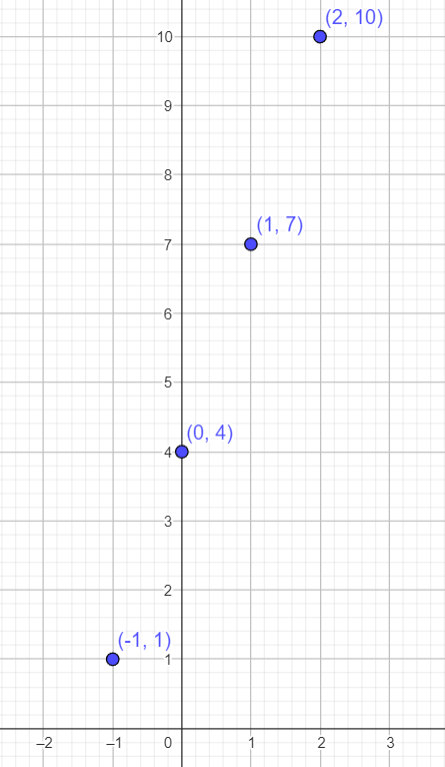
\includegraphics[scale=0.5]{img_26}



\subsection{Opgave 7}
17\% af 260kr

For at beregne 17\% af 260kr skal vi tage vores procenttal og dele det med 100, hvorefter vi ganger med beløbet. Vi har
\begin{align*}
\frac{17}{100}\cdot 260 = 0.17\cdot = 44.2
\end{align*}

17\% af beløbet 260kr er dermed 44.2kr.

\subsection{Opgave 8}

Hvor stor en procentdel er 20 ud af 270?

For at beregne hvor stor en procentdel 20 ud af 270 er, skal vi dividere de 20 med 270 og derefter gange med 100. Vi får

\begin{align*}
\frac{20}{270}\cdot 100 = 7.41
\end{align*}

20 er altså 7.41\% ud af 270.

\subsection{Opgave 9}
27 køer udgør 25\% af besætningen. Hvor stor er besætningen.

For at finde ud af hvor stor den samlede besætning er hvis 25\% af besætningen er 27 skal vi tage 100, dele det med procenttallet og gange det med besætningen. Vi har

\begin{align*}
\frac{100}{25}\cdot 27 = 108
\end{align*} 

Den samlede besætning er 108 køer.

\subsection{Opgave 10}
Løs ligningen $5+x=11$

For at løse ligningen skal vi isolere x dvs lade x stå alene på den ene side af lighedstegnet. Vi gør følgende

\begin{align*}
5+x &= 11\\
\Updownarrow\hspace*{2mm} &\\
5+x-5 = 11-5 && \text{trækker 5 fra på begge sider}\\
\Updownarrow\hspace*{2mm} &\\
x = 6
\end{align*}

Løsningen til ligningen er dermed $x = 6$.

\subsection{Opgave 11}
Løs ligningen $4x - 2 = 10$

For at løse ligningen skal vi isolere x dvs lade x stå alene på den ene side af lighedstegnet. Vi gør følgende

\begin{align*}
4x - 2 &= 10\\
\Updownarrow\hspace*{2mm} &\\
4x - 2 + 2 = 10 + 2 && \text{lægger 2 til på begge sider}\\
\Updownarrow\hspace*{2mm} &\\
4x = 12\\
\Updownarrow\hspace*{2mm} &\\
\frac{4x}{4} &= \frac{12}{4} &&\text{dividerer med 4}\\
\Updownarrow\hspace*{2mm} &\\
x = 3
\end{align*}

Løsningen til ligningen er deremd $x = 3$.

\subsection{Opgave 12}

Udregn følgende $4(2+a)$.

For at udregne ovenstående udtryk skal vi gange 4 tallet ind i parentesen. Når vi ganger tal ind i parenteser skal vi gange tallet ind på alle ledene i parentesen, i dette tilfælde skal vi gange 4 tallet ind på både 2 og a. Vi får

\begin{align*}
4(2+a) = 4\cdot 2 + 4\cdot a = 8 + 4a
\end{align*}

\subsection{Opgave 13}
Udregn følgende $(4+a)(2+b)$

Når vi skal gange 2 parenteser sammen skal vi gange alle ledene i den første parenten sammen med alle ledene i den anden parentes. I dette tilfælde skal vi altså gange 4 sammen med 2 og b, samt a sammen med 2 og b. Vi får

\begin{align*}
(4+a)(2+b) = 4\cdot 2 + 4\cdot b + a\cdot 2 + a\cdot b = 8 +4b + 2a + ab
\end{align*}

\subsection{Opgave 14}
Løs andengradsligningen $3x^2 +2x +2 = 0$

Vi aflæser først a, b og c værdierne ud fra formlen for den generelle andengradsligning $ax^2 +bx +c =0$.
Vi får

\begin{align*}
a&=3\\
b&=2\\
c&=2
\end{align*}

Vi beregner dernæst diskriminanten $d = b^2 - 4ac$ for at se om andengradsligningen har 2, 1 eller 0 løsninger.

\begin{align*}
d = b^2 -4ac = 2^2 -4\cdot 3\cdot 2 = 4 - 24 = -20
\end{align*}

Siden diskriminanten d er mindre end 0 altså $d<0$ har andengradsligningen ingen løsning. 

\subsection{Opgave 15}
Udregn $\frac{1}{2} + \frac{1}{8}$

For at addere 2 brøker skal brøkerne først have fælles nævner. I vores tilfælde har vi en brøk med nævneren 2 og en brøk med nævneren 8. For at de får fælles nævneren 8 skal vi altså gange med 4 i tælleren og nævneren på den brøk der har nævneren 2.

\begin{align*}
\frac{1}{2} + \frac{1}{8} = \frac{1\cdot 4}{2\cdot 4} + \frac{1}{8} = \frac{4}{8} + \frac{1}{8} = \frac{4+1}{8} = \frac{5}{8}
\end{align*}

\subsection{Opgave 16}
Udregn $\frac{1}{2}\cdot \frac{1}{8}$

For at gange 2 brøker sammen ganger vi deres tællere sammen og deres nævnere sammen. Vi får

\begin{align*}
\frac{1}{2}\cdot \frac{1}{8} = \frac{1\cdot 1}{2\cdot 8} = \frac{1}{16}
\end{align*}

\subsection{Opgave 17}
Udregn $\frac{1}{2}:\frac{1}{8}$

For at dividere en brøk med en anden kan vi i stedet for gange med den omvendte brøk. Den omvendte brøk er brøkken hvor der er byttet om på tælleren og nævneren.

\begin{align*}
\frac{1}{2}:\frac{1}{8} = \frac{1}{2}\cdot \frac{8}{1} = \frac{1\cdot 8}{2\cdot 1} = \frac{8}{2} = 4
\end{align*}
